%----------------------------------------------------
%
% Title:  Traverso 0.40.0
% Author: Remon Sijrier, Nicola Doebelin
% Date:   Januar 13, 2007
%
%----------------------------------------------------
% Created with TeXwiz 2.0.0
%----------------------------------------------------

\documentclass[a4paper,
               12pt,
               pdftex,
               twoside,
               smallheadings,
               headsepline,
               headinclude,
               DIV16,
               BCOR10mm
               ]{scrreprt}

\usepackage{mathpazo}
\usepackage[scaled=.95]{helvet}
\usepackage{courier}
\linespread{1.05}
\usepackage[latin1]{inputenc}
\usepackage{calc}
\usepackage{graphicx}
\usepackage{subfigure}
\usepackage{amssymb}
\usepackage{booktabs}
\usepackage{pdfpages}

%---------------- Page style options ----------------

\usepackage[automark]{scrpage2}
\pagestyle{scrheadings}

\setcapindent{1em}

%-------------- Custom Markup Commands --------------

\newcommand*{\FigB}{fig.}      % "fig." as used in brackets
\newcommand*{\FigT}{figure}    % "figure" as used in running text
\newcommand*{\FigsT}{figures}  % "figures" (plural) in running text
\newcommand*{\TabB}{tab.}      % "tab." as used in brackets
\newcommand*{\TabT}{table}     % "table" as used in running text
\newcommand*{\TabsT}{tables}   % "tables" (plural) used in running text

\newcommand*{\sact}[1]{$<$#1$>$} % single click action
\newcommand*{\dact}[1]{$\ll$#1$\gg$} % double click action
\newcommand*{\hact}[1]{{[#1]}} % single hold action

\newcommand*{\Version}{0.40.0} % The current version of traverso
\newcommand*{\Ubuntu}{7.04 Feisty Fawn} % The current Ubuntu version

%---------------- PDF output options ----------------

\pdfoutput=1
\usepackage{thumbpdf}
\usepackage[bookmarks]{hyperref}
\pdfimageresolution=300
\pdfcompresslevel=9

\pdfinfo{
/Title(Traverso 0.40.0)
/Creator(TeX)
/Producer(PdfTeX)
/Author(Nicola Doebelin)
/CreationDate(D:20070113145749)
/Subject(Traverso 0.40.0)}

%----------------------------------------------------

\renewcommand{\floatpagefraction}{0.6}
\renewcommand{\dblfloatpagefraction}{0.6}
\newcommand{\clearemptydoublepage}{\newpage\pagestyle{empty}\cleardoublepage}

% sloppy wordspacing:
\tolerance 1414
\hbadness 1414
\emergencystretch 1.5em
\hfuzz 0.3pt
\widowpenalty=10000
\vfuzz \hfuzz
\raggedbottom

\begin{document}


\title{Traverso 0.40.0}
\author{Digital Audio Workstation}
\date{\today}
%----------------- Custom title page ----------------

\begin{titlepage}
  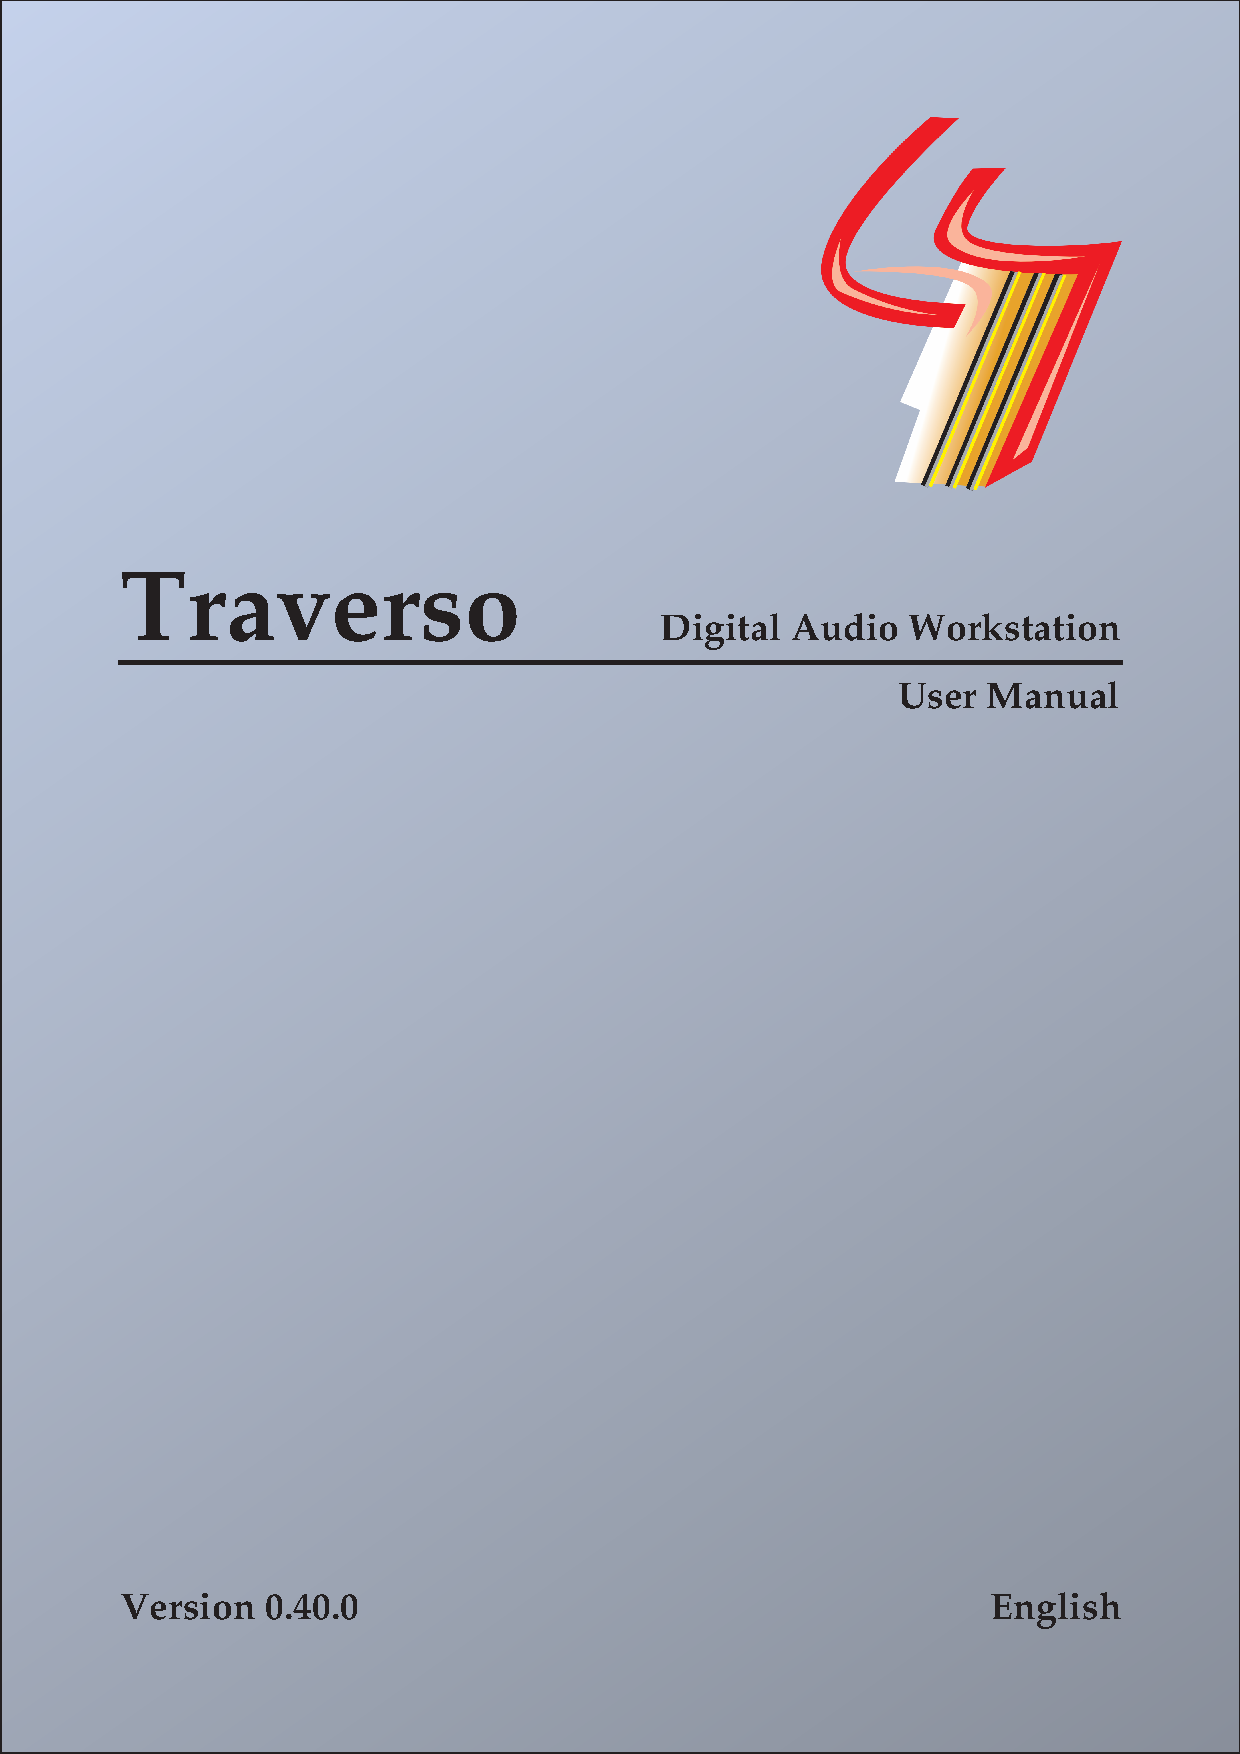
\includepdf{titlepage.pdf}
\end{titlepage}
  \clearemptydoublepage
  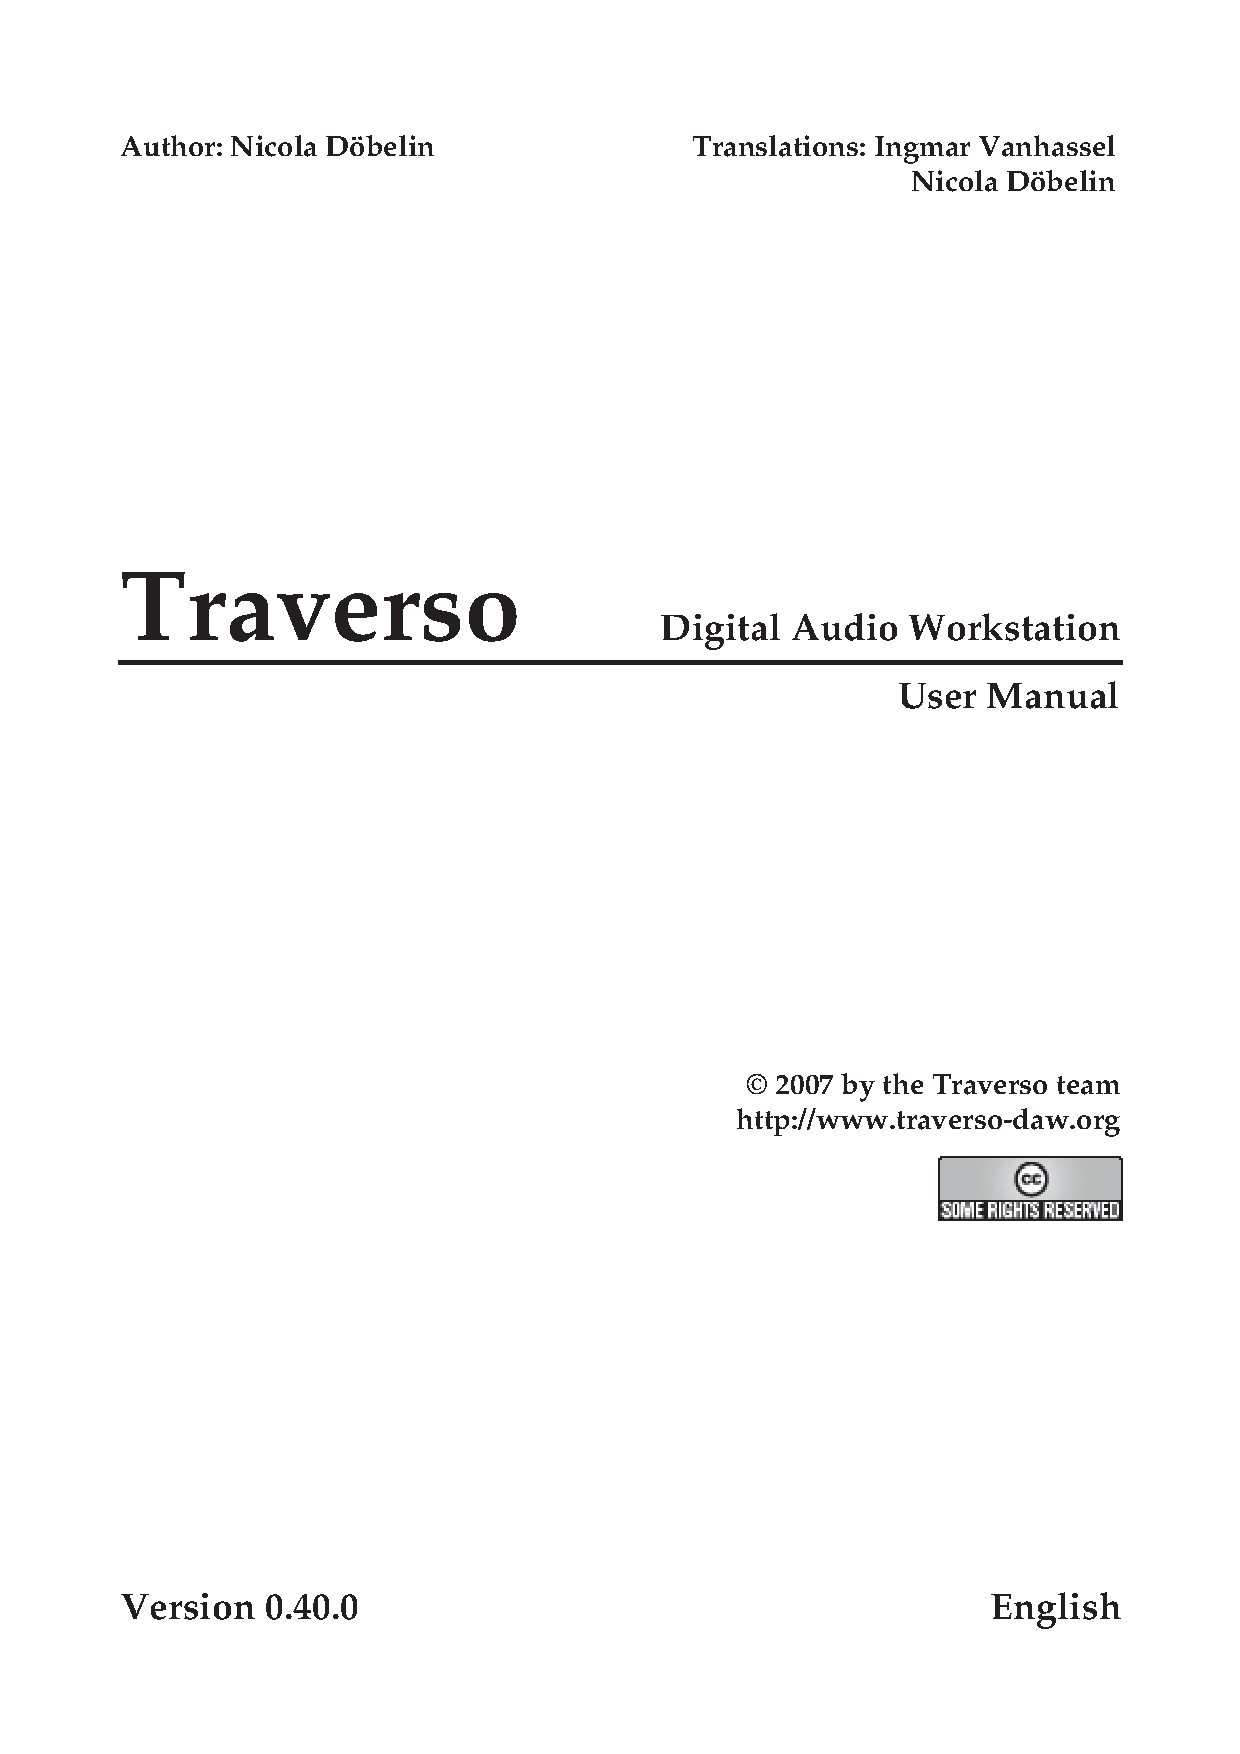
\includepdf{titlepage-author.pdf}

\clearemptydoublepage
\noindent\thispagestyle{empty}
This work is licensed under the Creative Commons Attribution-Noncommercial 2.5 Netherlands License. To view a copy of this license, visit http://creativecommons.org/ licenses/by-nc/2.5/nl/ or send a letter to Creative Commons, 171 Second Street, Suite 300, San Francisco, California, 94105, USA.\\\\
In short, you are free:
  \begin{itemize}
    \item \textbf{to Share} -- to copy, distribute and transmit the work
    \item \textbf{to Remix} -- to adapt the work
  \end{itemize}
  Under the following conditions:
  \begin{itemize}
    \item \textbf{Attribution.} You must attribute the work in the manner specified by the author or licensor (but not in any way that suggests that they endorse you or your use of the work).
    \item \textbf{Noncommercial.} You may not use this work for commercial purposes.
    \item For any reuse or distribution, you must make clear to others the licence terms of this work.
    \item Any of the above conditions can be waived if you get permission from the copyright holder.
    \item Nothing in this license impairs or restricts the author's moral rights.
  \end{itemize}
\normalsize


\clearemptydoublepage


\tableofcontents

%--------------- Start of the document --------------

\chapter{Introduction\label{sect_introduction}}
Traverso is a multitrack audio recording and editing program for GNU/Linux with special emphasis on an intuitive, clean, and above all efficient user interface. The program currently supports recording of any number of audio tracks (only limited by hardware capabilities), basic mixing features, and rendering of the  project into various standard audio file formats. The audio engine uses 32 bit floating point precision for all calculations to preserve the highest possible audio quality even after extensive processing.

The user interface uses a contextual interaction concept; instead of relying on the mouse to operate on graphical objects, combinations of mouse and keyboard are used to control the program. This results in a higher flexibility and much faster control of the program when compared to the traditional mouse-based approach. It even goes far beyond the possibilities offered by conventional key shortcuts. The mouse only has to be placed on an object and all functions become available instantly by pressing a key on the keyboard. Since the object under the mouse cursor is automatically selected, this concept is called ``soft selection''.

\section{License}
Traverso is free software; you can redistribute it and/or modify it under the terms of the GNU General Public License as published by the Free Software Foundation; either version 2 of the License, or (at your option) any later version.

This program is distributed in the hope that it will be useful, but WITHOUT ANY WARRANTY; without even the implied warranty of MERCHANTABILITY or FITNESS FOR A PARTICULAR PURPOSE.  See the GNU General Public License for more details.

You should have received a copy of the GNU General Public License along with this program; if not, write to the Free Software Foundation, Inc., 51 Franklin Street, Fifth Floor, Boston, MA  02110-1301, USA.

\section{Motivation}
One of the motivations to introduce the concept of soft selection was our belief in the superiority over the traditional point-and-click concept in regard to efficiency, speed, and ergonomics. The full potential of soft selections develops after an initial learning phase, because something that breaks with existing standards requires time and effort to adopt, and it takes even more time to overcome long-trained habits. But let's have a look at the different working styles with a trivial example. Suppose we want to do something as simple as switching ``Solo'' or ``Mute'' of a track on and off.

\minisec{The ``analogue way''}
In an analogue recording studio with a mixing desk, you have lots of channels, and each channel has lots of buttons, faders, knobs etc. To toggle ``Solo'' or ``Mute'', you identify the channel strip on the mixing desk, and press the corresponding button. If you want to do the same with several channels, you can quickly press many buttons in a row. The fact that there is a dedicated button for each and every function (which is not always trivial to find, depending on the size of the desk), makes it easy to switch the button, but results in mixing desks being huge and complicated electronic devices.

\minisec{The ``Digital Way''}
On a conventional digital audio workstation (DAW) you identify your channel and press the corresponding solo or mute button with the mouse. Depending on the user's skills and the size of the button, this can already be a minor challenge. Switching several channels in a row, however, is very slow and inefficient, because hitting the button requires careful positioning of the mouse cursor each time.

\minisec{The ``Traverso Way'': Soft Selection}
In Traverso you move the mouse over the track you want to process, and press a key on the keyboard, e.g. ``U'' for mute, or ``O'' for solo. Most users hit the key without looking at the keyboard. The track panel is a large area, which is entirely sensitive for the key actions, so even if several tracks should be switched, the mouse cursor can be placed anywhere on the track, requiring much less aiming.

So what is the difference between the digital and the Traverso way? From our experience, moving the mouse on the desk in order to move the cursor on the screen is like using a remote control or a ``finger extension''. It's like being allowed to press buttons on a mixing desk only by using a 30 cm long ruler. One would have to target carefully, and would miss the tiny button most of the time. All in all it would be very tiring and time consuming. Pressing buttons with our fingers, one for mute, one for solo etc., is more ergonomic and intuitive, and we tried to find an interface concept for Traverso which gives a feeling as direct as analogue buttons, without requiring additional hardware control surfaces. So once we have identified the channel we want to process (by hovering the mouse cursor over it), we want a real world button for as many functions as possible. And since our left hand could as well be ready on the keyboard instead of picking our nose, we have all the 104 buttons of our keyboard at our disposal which can give direct access to a large number of actions. This concept is closely related to the handling of action games (e.\,g. ``first-person shooters''), which are highly optimized for efficient and intuitive access to various actions (moving, running, shooting, ducking, \dots) and a large number of tools. To summarize, the advantages of soft selections are:

\begin{itemize}
 \item the distances on the keyboard are shorter than on the screen
 \item the hit-to-miss ratio for key strokes is much better than for buttons on the screen
 \item using both hands allows to work faster and relieves the mouse hand, resulting in a less fatiguing working style
 \item the ``remote control'' feeling is reduced
 \item more actions can be reached directly, requiring less and shallower menu structures
 \item the keys can be found blindly, leading to less distraction from the work flow
\end{itemize}

The downside is a steeper learning curve, particularly at the very beginning, since the keys are not labeled with the function name (``Solo'', ``Mute'', ``Rec'' etc.). But you will soon internalise the commands just as you did with ``Ctrl+C'' for copy and ``Ctrl+V'' for paste. As for the higher efficiency: Could you imagine driving your car, and when approaching a red light first having to open the menu ``brakes'' on your board computer, choose the sub-menu ``change hydraulic pressure'', and adjust the pressure for each wheel manually with the mouse?


\chapter{Installation\label{sect_installation}}
The most convenient way to install Traverso is to use one of the available installers. For Traverso \Version\ binary packages are available for several popular Linux distributions. However, in the fast-living open source world, things can change rapidly. It is thus recommended to refer to the Traverso homepage \cite{trav-hp} in order to find up-to-date information on binary packages. Alternatively, compilation from source is the second best option, and explained here in detail. It's actually quite simple as you will see! Traverso successfully builds and runs on i386, ia64, and ppc platforms.

\section{Binaries}
The precompiled binaries are available from the following locations:

\begin{description}
	\item [(K)Ubuntu:] The download page at \cite{trav-hp} has a debian package.
	\item [Gentoo:] Traverso is part of the official distribution. New versions of Traverso appear in the Pro-Audio overlay first. You'll find more info at \cite{pro-audio-wiki}.
	\item [SuSE:] Packages are available from \cite{suse-ref}
\end{description}

\section{Compiling from Source}
This section describes how to compile Traverso from source on a (K,X)Ubuntu \Ubuntu\ system. For other distributions, the package names may be somewhat different, but you should be able to identify the correct package with your distributions package manager. Note that Traverso depends on the Qt library version 4.2.3 or newer (4.3.1 recommended).

First you will need to make your system fit to compile Traverso. And while we're at it, install some more useful things. Use your favorite package manager (like synaptic or adept) to install the following packages:

\begin{itemize}
 \item libqt4-core, libqt4-gui, libqt4-dev
 \item libsndfile1, libsndfile1-dev
 \item libsamplerate0, libsamplerate0-dev
 \item libjack0.100.0-0, libjack0.100.0-dev
 \item libasound2, libasound2-dev
 \item fftw3, fftw3-dev
 \item jackd, qjackctl, gcc, g++, make
 \item build-essential
 \item (optional: libslv2, libslv2-dev from \cite{trav-repo})
\end{itemize}
On (K,X)Ubuntu the following will get you going:
\begin{verbatim}
$ sudo apt-get install build-essential libqt4-core \
 libqt4-gui libqt4-dev libsndfile1 libsndfile1-dev \
 libsamplerate0 libsamplerate0-dev libjack0.100.0-0 \
 libjack0.100.0-dev libasound2 libasound2-dev \
 fftw3 fftw3-dev jackd qjackctl gcc g++ make
\end{verbatim}
If some packages are not available, you should enable the universe repository. Instructions on how to add repositories are available for Kubuntu and Ubuntu on the distribution website and related forums / wikis.

In case you have version 3 of the Qt library installed (which is the default in (K,X)Ubuntu), you must make sure that the tools of version 4 are used. Open a terminal, enter the following commands and always select the Qt4 version when asked:

\begin{verbatim}
$ sudo update-alternatives --config qmake
$ sudo update-alternatives --config moc
$ sudo update-alternatives --config uic
\end{verbatim}

Now your system is ready to compile Traverso from source! Download the latest stable release of Traverso from the Traverso homepage. Extract it in some directory like /home/you/traversosource/ and compile it with the following commands:

\begin{verbatim}
$ tar -zxvf traverso-x.x.x.tar.gz
$ cd traverso-x.x.x
$ ./cleancompile
\end{verbatim}
(The cleancompile script ensures that all traces of previous compilations are removed, and calls qmake and make to start the new compilation.) This will take some time, and if you followed the instructions above carefully, it should run through without errors. When the make process has finished and you get back the  command line prompt, check the last 10 lines for the word ``Error''. If you don't find it, everything is ok. If you find it, check again if you followed the instructions above correctly. Now you can install the software by typing the following lines:

\begin{verbatim}
$ sudo make install
$ sudo echo /usr/local/lib >> /etc/ld.so.conf
$ sudo ldconfig
\end{verbatim}

\chapter{Key Actions\label{sect_keyactions}}
If the mouse points to a graphical object, some key command has to be performed, for example to mute an audio clip, or modify the gain of a track. A key command is a single key press, a combination of key presses, or a key hold action in combination with a mouse movement. Don't be afraid, this is not as difficult as it sounds! The following description shows how the different categories of key actions are notated and how they are performed.

\minisec{Single Key Action: Press and Release}
This action is noted as follows:
\begin{quotation}
   \sact{K}
\end{quotation}
This reads as: ``Press and Release a Key'', just like if you were typing in a letter.
``K'' is the key you should use. (\emph{Note:} Even though capital letters are used to write down these actions, you should just press the ``K'' key and never use shift or caps lock, unless it is explicitly mentioned.) For example:
\begin{quotation}
   \sact{F}
\end{quotation}
means press and release the ``F'' key.

\minisec{Single Key Action: Press and Hold}
This action is noted as follows:
\begin{quotation}
   \hact{K}
\end{quotation}
This reads as: ``Press and Hold the Key''. Pretty self explanotary, in a text editor you would get lots of kkkkkkkkkkk\dots.
Again, ``K'' is the letter associated with this action. For example:
\begin{quotation}
   \hact{D}
\end{quotation}
means press and hold the ``D'' key.

Hold keys in itself don't do anything. However if a ``hold key'' is active, and you move the mouse, an ``analogue'' action can be performed like moving an audio clip.

\minisec{Single Key Action: Press and Release Twice}
This action is noted as follows:
\begin{quotation}
   \dact{K}
\end{quotation}
It reads as: ``Press and Release the key twice''. Like typing in one letter twice, rather fast, like a double click. For example:
\begin{quotation}
   \dact{G}
\end{quotation}
means press and release the ``G'' key twice.

\minisec{Double Key Action: Press and Release}
This action is noted as follows:
\begin{quotation}
   \sact{K K}
\end{quotation}
This reads as: ``Press and Release 2 keys at once''. One of the more difficult actions. For example:
\begin{quotation}
   \sact{F G}
\end{quotation}
means press and release both the ``F'' and ``G'' key at the same time.

\minisec{Double Key Action: Press and Hold}
This action is noted as follows:
\begin{quotation}
   \hact{K K}
\end{quotation}
It reads as: ``Press and hold 2 keys at once''. For example:
\begin{quotation}
   \hact{F G}
\end{quotation}
means press and hold at the same time both the ``F'' and ``G'' key.

The same idea applies as for the ``Single Key Action: Press and Hold'', however you have to press and hold 2 keys. This is a bit more difficult to do than with a Single Key Action, and is meant for more advanced usages/users.

\minisec{Double Key Action: Press and Release Twice}
 This action is noted as follows:
\begin{quotation}
   \dact{K K}
\end{quotation}
It reads as: ``Press and Release the 2 keys twice''. A difficult action to learn. Two keys have to be pressed and released at the same time, twice rather fast after each other! For example:
\begin{quotation}
   \dact{F G}
\end{quotation}
means press and release both the ``F'' and ``G'' key at the same time twice.

This key command isn't used much actually, due the fact that it's rather hard to perform. But this makes it an ideal candidate for destructive actions!



\chapter{Setup\label{sect_setup}}
This chapter assumes that you have Traverso \Version\ or later installed on your system. If not yet so, please refer to chapter \ref{sect_installation} for instructions on how to install the programme.

Start Traverso from the application menu, or by hitting Alt+F2 and entering \texttt{traverso} in the command dialog. The first thing you will see is a file dialog asking you for the project directory. If you don't have one yet, create a new one. This directory will contain all projects, including the audio files. So be aware that if you want to do some serious audio work, you will need \emph{lots} of hard disk space. Change into the directory and press OK. After confirming your selection, the Traverso main window will be shown. It contains different regions which are sensitive for soft selections. The nomenclature used in this manual is shown in \FigT\ \ref{fig_gui01}.

\begin{figure}
 \centering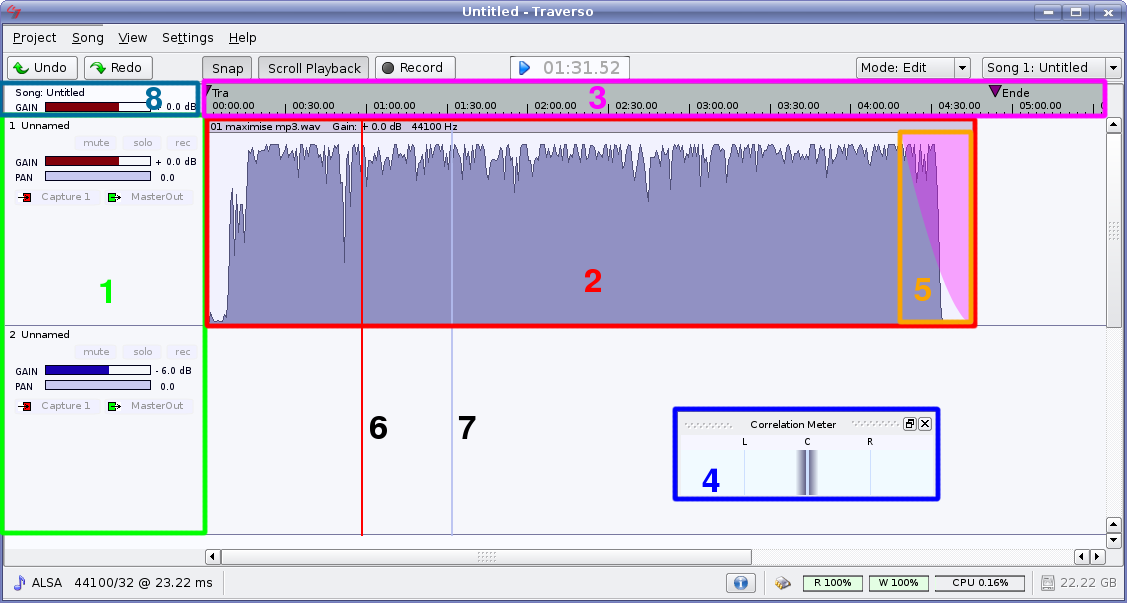
\includegraphics[width=\textwidth]{images/sshot06.png}
 \caption{Interface elements of Traverso: 1 Track panel:�If the mouse cursor is hovering over this area, all key actions apply to the track beneath it; 2 Audio clip:�Key actions apply to the audio clip; 3 Time line: Key actions apply to markers in the time line; 4 Dock window / Dock widget; 5 Fade out; 6 Work cursor; 7 Play head;�8 Song area.}
 \label{fig_gui01}
\end{figure}

Traverso uses dock windows for its tool dialogs, which allows to re-arrange the layout to your own liking. Just grab each one by the title bar and drag it to a new position. You can even stack the dock widgets on top of each other or detach from the main window and move freely. The latter is particularly handy with dual-screen setups, for the main window can occupy one screen, and the dock windows can be moved to the second screen (\FigB\ \ref{fig_mainwin02}).

\begin{figure}
 \centering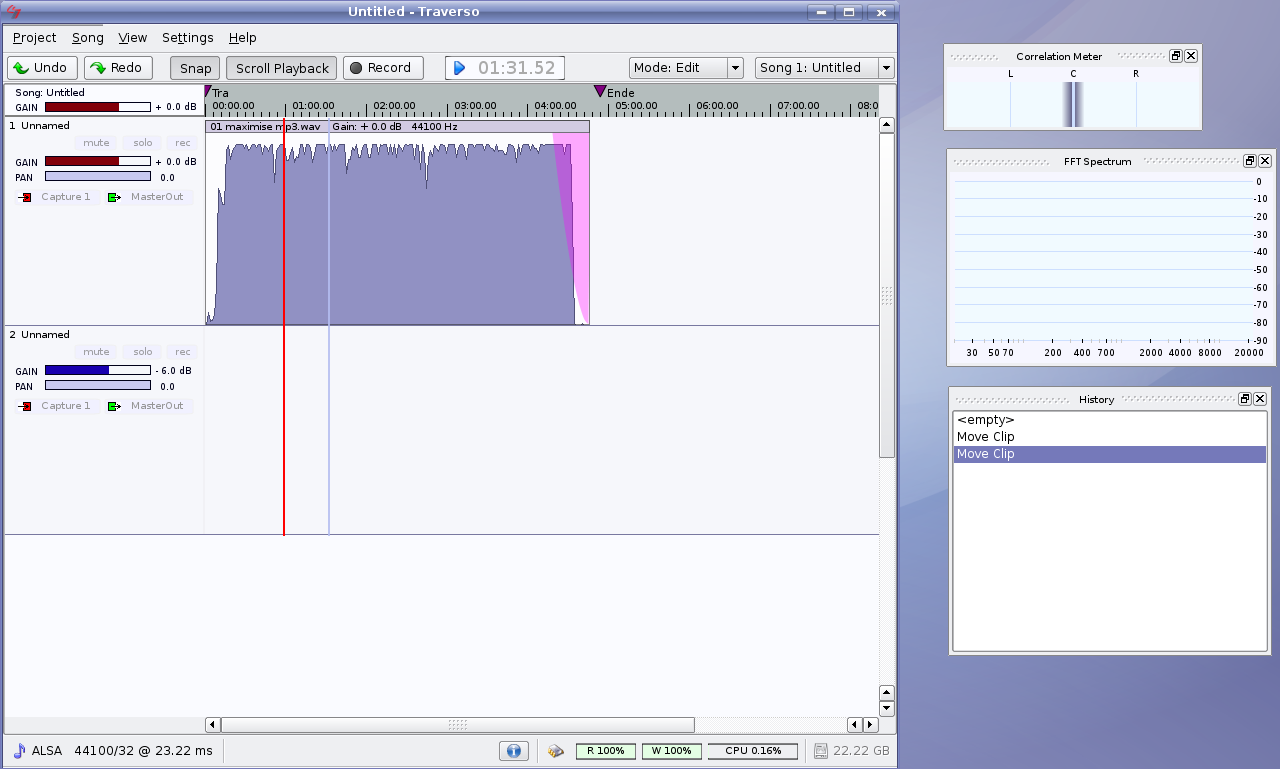
\includegraphics[width=0.9\textwidth]{images/sshot03.png}
 \caption{The dock windows can also be detached from the main window and moved to the second screen in a multi-screen setup.}
 \label{fig_mainwin02}
\end{figure}

\section{The Driver Backend}
Four driver backends are supported to date: The Null driver, ALSA, the jack soundserver, and Port Audio (on Windows and Mac OS�X). Let's have a look at all of them, what the advantages and disadvantages are, and how to set them up correctly. The currently loaded driver is displayed in the menu bar.

\subsection{Null Driver}
The Null driver is a fallback solution which is set if no other driver is available, but you won't hear any output as long as the Null Driver is loaded. Hence there's hardly a situation where you want to load it manually. To select a valid driver, click on the \emph{Null Driver} label in the menu bar to open a configuration dialog (\FigB\ \ref{fig_driverconf}).

\subsection{ALSA}
If ALSA is selected, Traverso communicates directly with the ALSA layer, which is only possible if no other application occupies the sound system. So before selecting ALSA as your driver, make sure you stop playback of all other sound applications. Also check the KDE/Gnome system tray for minimized instances of amarok, XMMS, etc. Back in Traverso's driver configuration dialog set the driver to \emph{ALSA}, the rate to 44100, and leave the latency. Then press \emph{Save} and \emph{Apply} and check if the entry in the menu bar has switched to \emph{ALSA}. If it refuses to load the new driver, your sound card may still be occupied by another application, so check again if you correctly stopped all multimedia applications and make sure that the sound daemon (e.\,g. aRTs) shuts down automatically when not used. Then try again to set the driver to ALSA. If it was accepted as a valid driver, the sound driver is set up correctly.

\subsection{Jack}
Traverso can also connect to the jack soundserver, which provides advanced routing features and zero-latency connections between clients. If you don't want to use these features and ALSA works for you, there's no advantage in using jack. We recommend to use \emph{qjackctl}, which allows to easily setup jack for your system. Start the jack daemon by pressing \emph{Start} in qjackctl. When it is running, set the driver in Traverso's configuration dialog (\FigB\ \ref{fig_driverconf}) to \emph{jack} and press \emph{Save} and \emph{Apply}. The menu bar should display \emph{jack} if the driver was loaded correctly. Now go back to qjackctl and open the \emph{Connect} dialog. \emph{Important:} You must set up the connection manually, otherwise you won't hear any sound. Select the Traverso entry in the left part (``Readable Clients''), and alsa\_pcm in the right part (``Writable Clients''), then press \emph{connect}. If a line connecting the two clients is drawn, the sound system is set up correctly.

\begin{figure}
 \centering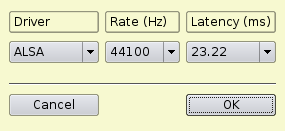
\includegraphics[width=0.5\textwidth]{images/sshot02.png}
 \caption{The audio driver backend can be selected from the menu bar. Traverso supports ALSA, jack, and PortAudio, and has a \emph{Null Driver} as fallback solution if no working driver is available.}
 \label{fig_driverconf}
\end{figure}

\subsection{Port Audio}
Port audio is the only driver backend available on Mac OS X and Microsoft Windows. It connects to the system's native sound system (CoreAudio on OS X, WMME on Windows). Simply select ``PortAudio'' in the driver configuration widget, the samplerate you wish to use, and a latency that works for you.

\chapter{Quick Start\label{sect_quickstart}}
The default project automatically created by Traverso contains six empty tracks and is called \emph{Untitled}. So how should we get started?
Let's just start Traverso and import an file to work on.

You will need a wave audio file, or better a couple of them. You can import them from any location on your hard disk, or place them in your Traverso project directory, and further in "Untitled/audiosources" to keep you directories tidy. Back in Traverso, press the I key on an empty track, navigate to the wave files in the file dialog, and select one of them. It will be placed in the track, and after a couple of seconds the wave form will be drawn (it takes a few seconds to calculate the wave form the first time).

We start listening to our imported audio file, by pressing the spacebar, the VUMeters will show the level of the output signal. If the VUMeters are not visible, show them from the menu ``Views $\rightarrow$ VUMeters''. Muting the audio clip is done by pressing the U key while the mouse points to the audio clip. To unmute the clip, press U again. To make life easier, throught this manual we use this notation for pressing the U key: \sact{U}. So, whenever you see a letter enclosed in these brackets, it means press that key once. If you point the cursor to the track background and press \sact{U}, the entire track is muted---and finally the ``mute'' button lights up!

OK, what about splitting our clip into half? Point the mouse to where you want your clip split, and press X, the shorthand notation then will be \sact{X}. All of a sudden we have two clips! Use the undo button in the menu bar to undo the latest action. The clip will return to it's previous state.

Changing the gain of a track or audio clip is done as follows: Point your mouse to the audio clip, and press and hold the G key! The cursor will change to a gain symbol (\FigB\ \ref{fig_gaincursor}). Now move the mouse up/down, and see the gain value change. To make live easier again, the shorthand notation for keys that are pressed \emph{and} held is \hact{G}. When releasing the G key, the cursor returns to it's normal state, and the new gain value will be used. If you point the cursor to the background of the track, e.\,g. between two clips or to the track panel on the left (where the ``Solo'', ``Mute'', and ``Rec'' buttons are), holding \hact{G} and moving the mouse will change the gain of the entire track. Instead of moving the mouse, try scrolling with the mouse wheel while holding \hact{G} to change the gain in very small steps. These actions, as you can see in the History view, are also un/redoable. You can also select an entry in the history view to jump directly to a certain state in the history.

\begin{figure}
 \centering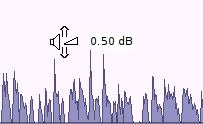
\includegraphics[width=0.4\textwidth]{images/gain-cursor.png}
 \caption{The cursor changes to a gain symbol during the \hact{G} action.}
 \label{fig_gaincursor}
\end{figure}

Up to now we used some simple and easily memorable actions, but there are of course a lot more. But how to know which functions are available for a track or audio clip? Fortunately, there are menus available. You can either use the righ mouse button to popup the menu for the object beneath the mouse cursor, or use \sact{Q} (by now you know that this means pressing the Q key). The menu shows the available functions, and how to perform them on the keyboard (\FigB\ \ref{fig_clipmenu})!

\begin{figure}
 \centering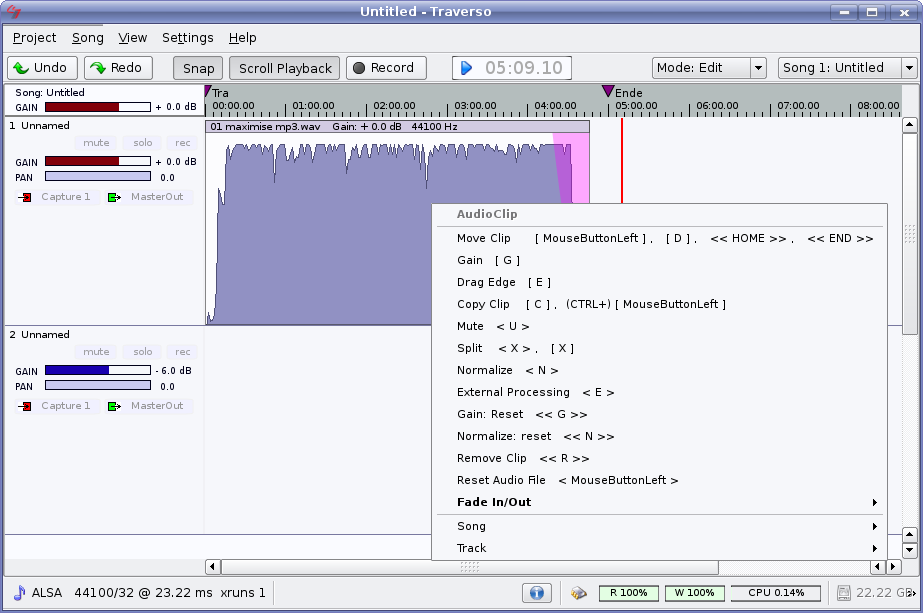
\includegraphics[width=\textwidth]{images/clipmenu.png}
 \caption{Pressing \sact{Q} or the right mouse button on an audio clip shows a menu with all available actions.}
 \label{fig_clipmenu}
\end{figure}

Moving the audio clip can be done by pressing the left mouse button, and keeping it pressed, or by doing the same with the D key. According to our notation scheme that would be \hact{D} or \hact{Left MouseButton}. Alternatively, you can just drag the audio clip with the mousecursor. You can move the mouse freely to position the audio clip to your own liking, the view will automatically scroll if the mouse comes close to the boundaries of the view. Also check out the \hact{Z} and \hact{S} actions to zoom and move the horizontal slider.

By now we learned two kinds of actions, the single key actions \sact{K}, and the hold actions \hact{K}. We also learned that key actions always work on the object beneath the mouse cursor. But before you start exploring the possibilities of Traverso on your own, let's look at some more (randomly selected) functions.

If you want to reset the gain of an audio clip or track to 0 dB, point the mouse cursor to a clip and press the G key twice. This works just like double-clicking with the mouse. In our notation scheme, a double key stroke is notated as \dact{G}. You will see that this action first resets the gain to 0 dB, and if called again, toggles the gain between $-6$ and 0 dB. This also works on the track gain.

As a last example let's delete an audio clip. First select the clip by hitting \sact{S} on it. Its background will become dark. Then hit X and C twice at the same time. This action is difficult to perform, maybe you need a couple of attempts to get it right. But this makes the action ideal for ``dangerous'' function which should by no means happen accidentally. According to our notation scheme this function writes as \dact{X C}. An overview of all available action types is given in chapter \ref{sect_keyactions}. Chapters \ref{sect_recording} and \ref{sect_mixing} provide more detailed information on recording and mixing.


\chapter{Recording\label{sect_recording}}
\section{Creating a new project}
To make some test recordings we first create a new project. Start Traverso and select ``New\dots''. Enter a name, set the number of songs to 1, the number of tracks to 2, and leave the rest empty. Then press ``OK'' to create the project and show it's first song. Note: All recorded audio data will be stored in \texttt{project\_dir/project\_name/audiosources}, so if you followed our advice and selected a project directory on a pratition with lots of free space, you shouldn't run out of disk space now.

\section{Setting up the driver}
To set up the driver backend, open the preferences dialog by clicking ``Settings $\rightarrow$ Preferences\dots'' (\FigB\ \ref{fig_driversettings}). Which driver is appropriate for your system is described in chapter \ref{sect_setup}. In the driver configuration one can chose the sampling rate, and Traverso always uses the sampling rate of the driver backend for its recordings. Traverso's audio engine works entirely in 32 bit floating point precision, and it uses standard wave files with 32 bit float precision to store recorded audio data.

\begin{figure}
 \centering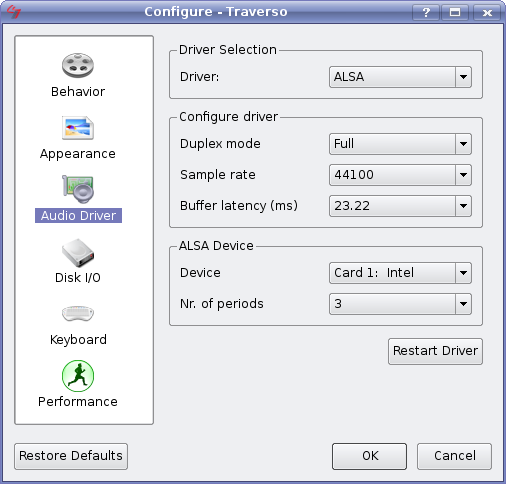
\includegraphics[width=0.75\textwidth]{images/driversettings.png}
 \caption{In ``Settings $\rightarrow$ Preferences\dots'', all driver related parameters can be set.}
 \label{fig_driversettings}
\end{figure}

\section{Recording}
Make sure a sound source is connected to the line-in bus of your sound card, and also make sure it really is playing back. In Traverso hit \sact{B} on the first track and select ``Capture 1'' as input bus, then hit \sact{A} to arm the first track. As soon as the track is armed, you should see the VUMeter indicating an input signal on Capture1. If not, the problem is most probably to be searched outside of Traverso. If you are sure your cable connections are correct, open KMix or a similar mixer applet to configure your sound card. As shown in \FigT\ \ref{fig_kmix01}, the Line and Capture channels had to be armed and un-muted on our test system before the line-in signal got through to Traverso.

\begin{figure}
 \centering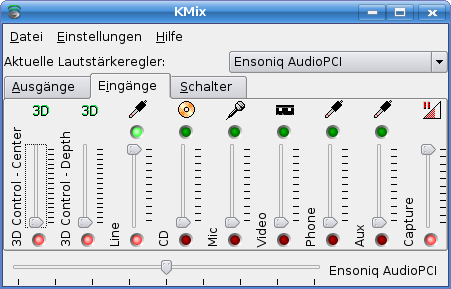
\includegraphics[width=0.8\textwidth]{images/kmix01.png}
 \caption{KMix can be used to configure the sound card. Make sure the correct input channels (Line and Capture) are un-muted and set for recording (green and red buttons).}
 \label{fig_kmix01}
\end{figure}

When you are ready to record, press the \texttt{Record} button in the title bar or hit CTRL+\sact{SPACE} to start the recording, and hit \sact{SPACE} to stop recording. That's it. In order to rehearse the recording, place the work cursor before the newly recorded clips, and press \sact{SPACE} to start playback. Once you have finished recording a track, don't forget to unarm it by pressing \sact{A}, or unarm all armed tracks at once by hitting \dact{A}.


\chapter{Mixing\label{sect_mixing}}
Mixing features in Traverso \Version\ currently include gain, panorama, different fade shapes for fade-in and -out, trimming, splitting, moving of audio clips, and gain curves. An infrastructure for effect plugins using the LV2 standard is implemented, but development of Traverso \Version\ is a bit ahead of LV2, hence no plugins are available at the moment of writing. Starting from version 0.40.0, Traverso has basic support for using Sox to process audio clips.

\section{Moving, trimming, splitting}
Clips can be moved freely by holding \hact{D} and moving the mouse. If snapping is active (\sact{S~N}), both ends of the dragged clip will snap to the beginning of the song, edges of other clips, and to the work cursor.

Move the mouse cursor on a clip, hold \hact{E}, and move the mouse horizontally to drag the edge of the clip which is nearest to the mouse position. If snapping is active, the edge will snap to the positions described above.

Audio clips can be split by pointing the mouse cursor to the desired position and pressing \sact{X}. Of course the edges of the two clip fragments can be fine-tuned by holding \hact{E} as describes above.

\section{Fades}
Both ends of a clip can be faded smoothly by holding \hact{F} on the left or right half of the clip and moving the mouse horizontally. On the left half the key action refers to the fade-in, on the right half it refers to the fade-out. Several fade shapes are available, which can be toggled by \sact{M} (\FigB~\ref{fig_fades01}).

\begin{figure}[t]
 \centering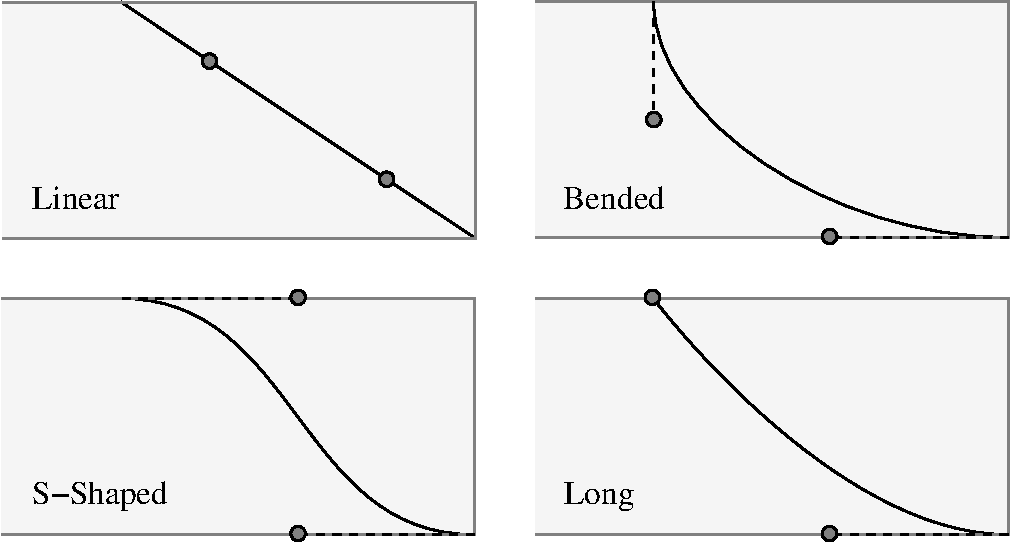
\includegraphics[width=0.8\textwidth]{images/fades}
 \caption{Different fade shapes are available in Traverso. Fade curves are defined as splines with two control points (circles) which can be modified by the values ``bending'' and ``strength''.}
 \label{fig_fades01}
\end{figure}

All shapes are based on a cubic spline curve with four knots. Two knots define the bending of the non-linear shapes. The positions of these control knots can be modified by two values ``bending'' and ``strength''. ``Bending'' defines the direction of the tangent in the end point, whereas ``strength'' changes the weight of the tangent (\FigB~\ref{fig_fades02}). It is not possible to move the control knots freely and independently, instead Traverso knows several modes which are relevant for fade shapes (\FigB~\ref{fig_fades01}):

\begin{figure}[t]
 \centering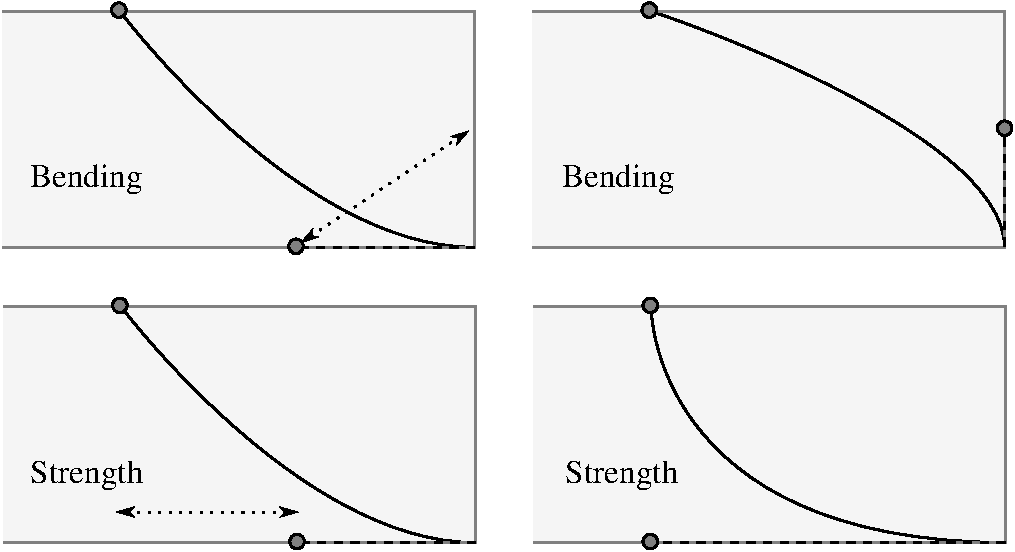
\includegraphics[width=0.8\textwidth]{images/fades2}
 \caption{Bending and strength values can be used to alter the shape of the fade curves. (Demonstrated with the ``Long'' mode.)}
 \label{fig_fades02}
\end{figure}

\subsection{Linear}
Linear fades are a straight line between the start and end point. The control knots can't be changed. Linear fades tend to sound rather abrupt at the low-level end of the fade, and are thus not the preferred mode for long fade-outs, e.\,g. at the end of a song.

\subsection{S-shaped}
The S-shaped mode starts with a horizontal tangent, is steep a the center, and passes into a horizontal tangent again. The beginning and end are very smooth, but the center part can sometimes change too quickly in short S-fades. The ``strength'' parameter can be used to soften the center part and make the volume change less obvious. The ``bending'' factor should usually remain between linear and horizontal tangents, however, vertical tangents can be used for effects.

\subsection{Bended}
The bended mode acts similar to the S-shaped mode, but the control knots point to the same side. This mode can be used to achieve a very fast volume drop at the beginning of the fade-out, and very soft towards the end. Both control parameters are useful to find the best balance between a beginning that is not too fast, and an ending that is still slow enough for a soft fade-out effect.

\subsection{Long}
The long mode only allows to change the control knot at the low-level end of the fade. This mode is often used for very smooth fade-outs, e.\,g. at the end of a song. The high-level end changes fastly, but the low-level tail is very soft. The long mode often sounds more musical than a similar bended mode.

\section{Gain curve}
Gain curves are a powerful feature to change the gain of an audio clip in the time line. The curves are child elements of audio clips, therefore their \emph{relative} position to the audio clip will always stays the same. To change to effects mode, select the entry ``Mode: Effects'' from the dropdown menu in the menu bar (\FigB~\ref{fig_gcurve01}). To change back to edit mode ``Mode: Edit''. A default curve node is added automatically at the beginning of the clip at 0~dB. Additional nodes can be created by \dact{C} at the position of the mouse cursor. Nodes can also be dragged (\hact{D}) and removed (\dact{R}). These actions always apply to the node closest to the mouse cursor, which is indicated by a different colour.

\begin{figure}[t]
 \centering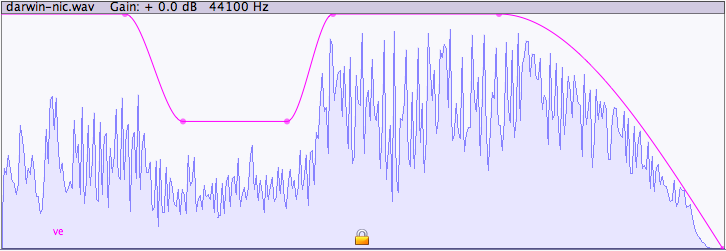
\includegraphics[width=\textwidth]{images/gcurve01}
 \caption{The ``effects mode'' of Traverso can be activated from the dropdown menu in the menu bar. Gain curves are only visible in that mode. Nodes can be added, removed, and dragged freely.}
 \label{fig_gcurve01}
\end{figure}

\section{Plugins}
Traverso supports the LV2 plugin interface, which is the successor of the LADSPA standard. Plugins can be added to tracks by pressing \sact{F5}, which opens a list of all LV2 plugins installed on the system (\FigB~\ref{fig_pluglist}). Active plugins will be shown as semi-transparent fields in the track view. These fields have their own context menu; just try it out by holding the mouse on them and pressing \sact{Q}. Pressing \sact{E} will open a generic dialog, which allows to adjust the plugin parameters. Plugins can also be bypassed (\sact{B}) and removed (\dact{R}). Version 0.40.x inserts all plugins post-fader. More flexible solutions will follow in upcoming versions.

\begin{figure}[t]
 \centering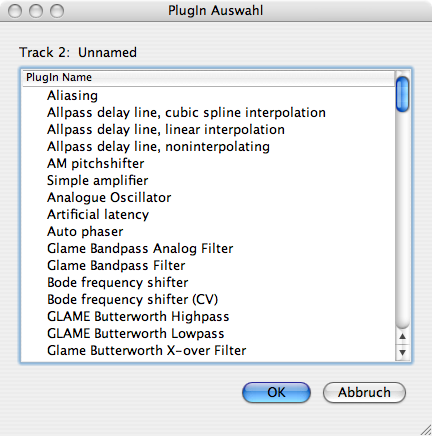
\includegraphics[width=0.6\textwidth]{images/plugin-list}
 \caption{Plugins can be added to a track by pressing \sact{F5}.}
 \label{fig_pluglist}
\end{figure}



\chapter{Laying out a CD\label{sect_cdburning}}
\section{Requirements}
This chapter describes how to arrange and write a Red Book compatible audio CD. Traverso uses \texttt{cdrdao} to actually write the CD, so this program must be installed on the system. \texttt{cdrdao} is available from the official repositories of all  major and up-to-date Linux distributions, it is thus recommended to install it via the distribution's package manager. The Windows and Mac OS X installer takes care of installing cdrdao for you, so if you are on one of these platforms, you skip this section!

\footnotesize
\begin{verbatim}
tux@linux:~$ cdrdao

Cdrdao version 1.2.2 - (C) Andreas Mueller <andreas@daneb.de>
  SCSI interface library - (C) Joerg Schilling
  Paranoia DAE library - (C) Monty

Check http://cdrdao.sourceforge.net/drives.html#dt for current 
driver tables.


Usage: cdrdao <command> [options] [toc-file]
command:
...
\end{verbatim}
\normalsize

If the command was not found, the next section explains how to install \texttt{cdrdao} on the Linux platform.

\subsection{Linux}
Installing \texttt{cdrdao} on Linux is straight forward, since it is part of all major distributions. Use your distribution's package manager (e.\,g. Synaptic or Adept on (K)Ubuntu, Yast on SuSE), search for \texttt{cdrdao} and install the binary package. Alternatively, you can install it from a terminal. The commands will differ depending on the distribution. For (K,X)Ubuntu, enter the following lines in a terminal:

\begin{verbatim}
sudo apt-get update
sudo apt-get install cdrdao
\end{verbatim}


\section{Tracks and Markers}
There are basically two ways of defining tracks for a CD. Each sheet can be a track, or the entire CD can be arranged in the timeline of a sheet and tracks are defined by markers. Combinations of the two ways are also possible. Let's have a closer look at these two concepts.

\subsection{A Sheet is a CD-Track}
As you may have noticed, Traverso allows to have several sheets in a project. Some people like this feature, as one can combine all sheets of an album in one project, and still focus on one sheet at a time. If you want to write a CD containing all sheets of your project, make sure you check the ``All sheets'' button in the export dialogue. Each sheet will be rendered to a track, from position 00:00:00 up to the end of the last audio clip, and consequently each sheet will become a track on the CD.

\subsection{CD in a timeline}
Sometimes it is important to fine-tune the transition from one track to the next, e.\,g. by adding a little bit of silence in between, or by fading the previous track into the next one. In that case it can be easier to arrange the entire CD in one timeline and split it into tracks using markers. Let's look at an example in order to show how this works. (Look at \FigT~\ref{fig_markers01} if you get lost with the explanations.) Open or create a project with only two audio clips. Suppose we want clip 1 to be track 1 on the CD, and clip 2 will be track 2. Position them on the first and maybe second track, starting at position 00:00:00, as you want to hear them on the CD. Leave some silence between the end of clip 1 and the beginning of clip 2. To get Traverso to start a new CD track there, position the mouse cursor on the gap between the two clips, and press \sact{M}. This adds a small triangle to the timeline at the position of the mouse cursor, and two more at position 00:00:00 and at the end of clip 2. The latter one is labelled ``End'', and it marks the end of the CD. You can shift it a bit further back if you don't want the CD to stop right there (remember you  can have reverb tails extending beyond the last audio sample, which you don't want to cut off).

\begin{figure}[t]
 \centering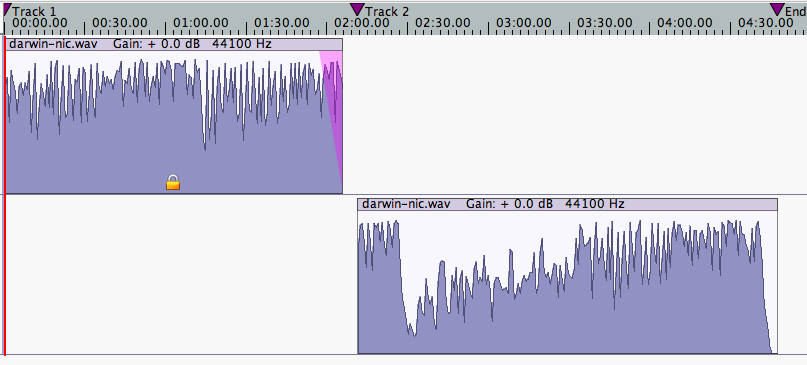
\includegraphics[width=\textwidth]{images/markers01}
 \caption{If a CD is arranged in one sheet, markers can be used to define CD tracks. Always keep the ones at position 00:00:00 and at the end.}
 \label{fig_markers01}
\end{figure}

These triangles are CD track markers, and they can be moved, added, and deleted freely (press \sact{Q} on the timeline to list all available functions.) However, it is also possible to create setups which don't make sense. E.\,g. only having one track marker in the timeline. In such cases, Traverso tries to guess the most sensible solution, and adds markers on the fly at positions it considers appropriate (which is usually at position 00:00:00 and after the last sample of the sheet containing audio data). Traverso also supports CD-text, which can be entered in the marker dialogue ``Views $\rightarrow$ Marker Dialog'' (\FigB~\ref{fig_marker-editor}). It is also possible to export the table of contents of the CD as an HTML file from this dialog. Album-wide CD-text can be entered in the project settings, opened from ``Project $\rightarrow$ Project Manager'', in the tab ``CD Text''.

\begin{figure}[ht]
 \centering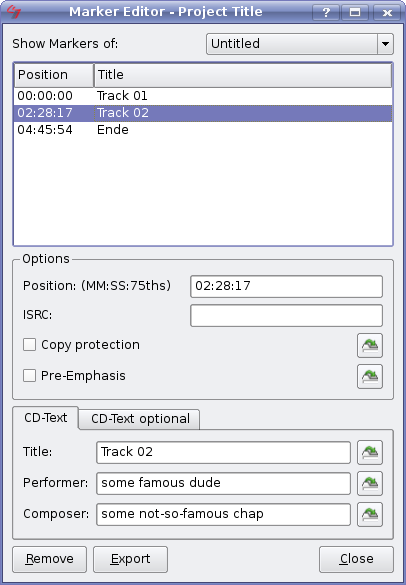
\includegraphics[width=0.45\textwidth]{images/marker-editor}
 \caption{The marker dialogue opened from ``Views $\rightarrow$ Marker Dialog'' allows to add CD-text, modify the markers, and export the table of contents as an HTML file.}
 \label{fig_marker-editor}
\end{figure}

Once the CD is laid out to your satisfaction, press \dact{RETURN} on the sheet to open the export dialogue (\FigB~\ref{fig_exportdlg}). You can either choose to export the project as audio files to the harddisk, or burn a CD. If you want to export to harddisk, you can choose between several audio formats. The most common one is WAVE, and depending on your plans with the exported files, you can use different sample formats (bit depths). 16 bit is ideal if you want to burn the files on CD later on. If you want to go on processing the files, use 32 bit float format instead. If you want to archive the files, use the FLAC codec, which is a lossless compression format.

If you want to burn a CD, you must also decide if you want to burn the current sheet (using markers to define CD tracks), or the entire project (each sheet becomes a track). If you check ``Export to disk only'', no CD will be written, but only a *.toc file and *.wav files for \texttt{cdrdao}.

Note for OS X users: CD writing support is still experimental. You can choose between several burning devices: IODVDServices, IODVDServices/2, IOCompactDiscServices, IOCompactDiscServices/2. These are hard-coded, so you probably don't have all of them installed. IOCompactDiscServices should only be used for old drives without DVD reading support. If you have multiple DVD drives, use IODVDServices or IODVDServices/2 to access the first and the second drive. In most cases IODVDServices will be the only working solution.

\begin{figure}[t]
 \centering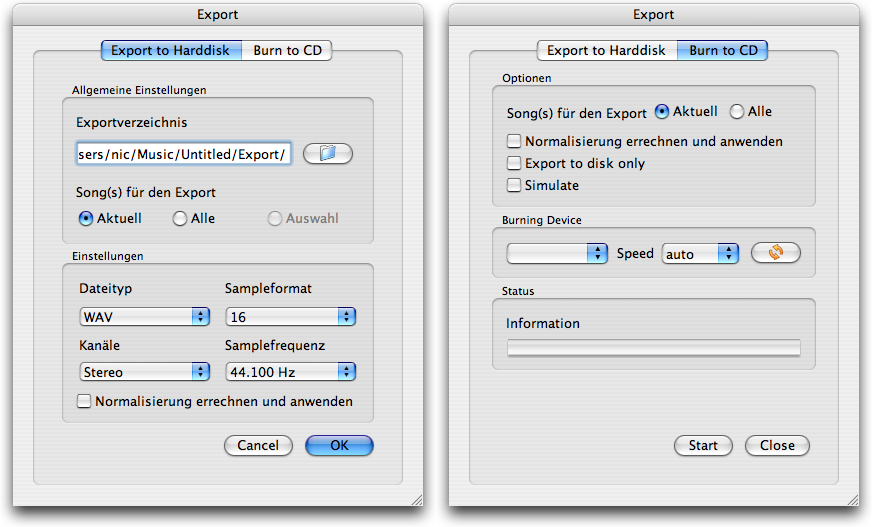
\includegraphics[width=\textwidth]{images/exportdlg}
 \caption{\dact{RETURN} opens a dialogue to export the project (either the current sheet or the entire project) to audio files, or burn a CD.}
 \label{fig_exportdlg}
\end{figure}


\chapter{Tools\label{sect_tools}}
\section{Correlation Meter}
The correlation meter monitors the stereo output of Traverso and displays the correlation coefficient of the left and the right channel signal. Unlike many other correlation meters it interprets the coefficient as a measure for stereo width and draws a gradient representing the stereo field.

In order to explain what correlation is and why it is important, we assume that a pure sine wave is played back on both the left and the right master channel. When both signals are merged (which happens if the signals are played back in mono), the resulting signal is the sum of the left and the right channel. Depending on the phase difference between the source signals, interference effects occur. That is, if two positive amplitudes are summed, the absolute value is greater, whereas if a positive and a negative amplitude are summed, the absolute value becomes smaller. In some cases this can lead to complete extinction, leaving nothing but a silent signal (\FigB\ \ref{fig_interference}).

\begin{figure}
	\centering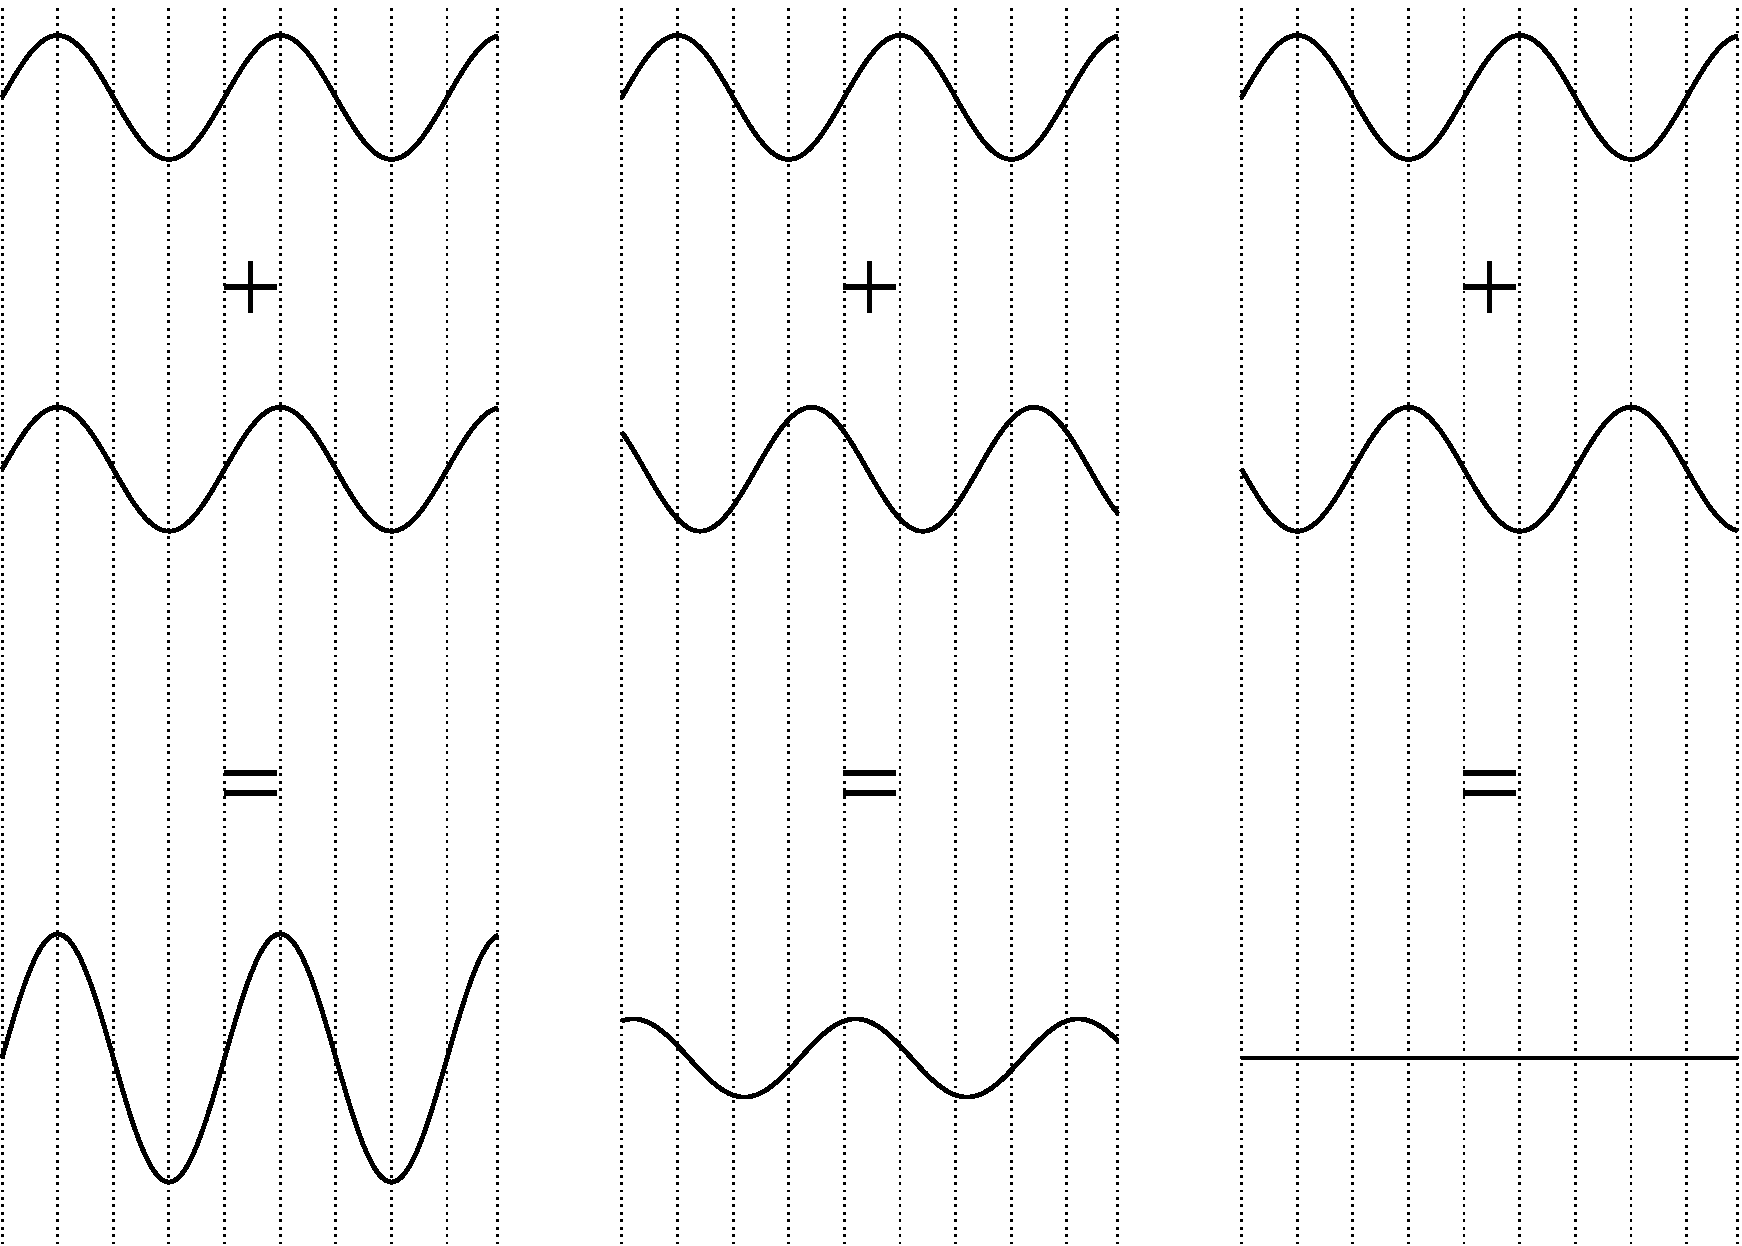
\includegraphics[width=0.8\textwidth]{images/sine01}
	\caption{When summing up two sine waves, interference can either lead to amplification (in phase, left), remain more or less unchanged (uncorrelated, middle), or lead to extinction (out of phase, right).}
	\label{fig_interference}
\end{figure}

If the two audio signals contain more complex data, e.\,g. music or spoken word, such extinction effects (also known as \emph{phase cancellations}) do not cancel out the entire signal, but merely certain frequencies, leading to a ``hollow'' or otherwise strange sound. Needless to say that such effects are rather devastating for a high quality audio production. Although it is indisputable that we should use our ears and listen to the mono signal in order to detect phase problems, computer based audio workstations allow to provide visual feedback of the audio data in many ways, which is one of the reasons for many users to prefer digital audio workstations. There are several ways to visually represent the correlation, but in order to understand how to interpret Traversos correlation meter, some more theory is required.

The amount of correlation is represented in the \emph{linear correlation coefficient} $r$, which is calculated over an array of pairs of samples $(x_i,y_i)$:
\[
r = \frac{\sum\limits_{i}(x_i - \bar{x})(y_i - \bar{y})}{\sqrt{\sum\limits_{i}(x_i - \bar{x})^2} \sqrt{\sum\limits_{i}(y_i - \bar{y})^2}}
\]
$r$ ranges from $-1.0$ to $1.0$. A value of $r = 1.0$ means the left and right signal are perfectly correlated. The master signal would be mono in that case, since there is no phase difference between the left and the right signal. The more difference there is between the two channels, the lower the correlation coefficient becomes. In case of totally uncorrelated data (which could read as ``no phase similarity whatsoever between the left and right channel''), $r$ becomes 0.0. Such a signal produces a wide stereo image with a low risk of phase cancellations when summed to mono. The difference between the signals can be further ``increased'' by one channel becoming the inverse of the other. In that case $r$ becomes $-1.0$. Negative $r$ values indicate high risk for phase cancellations.

The correlation meter of Traverso (menu ``Views $\rightarrow$ Correlation meter'') uses an intuitive way to display the correlation coefficient. Instead of focusing on the numerical value, it shows it's meaning in terms of stereo width (\FigB\ \ref{fig_cmeter01}). A gradient spreading between the left and the right speaker (marked by the L and R lines) indicates totally uncorrelated signals ($r = 0.0$) and thus a very wide stereo image. As long as the gradient does not extend beyond the L and R lines, there is no negative correlation and hence a low risk for phase cancellations. However, if it \emph{does} extend beyond the lines, phase cancellations are likely to occur if the signal is summed to mono, and the stereo image sounds unnaturally wide. This should be avoided by all means. A mono signal, on the other hand, causes the gradient to collapse to a line in the center.

\begin{figure}
	\centering
	\subfigure[Stereo, $r = 0.0$]{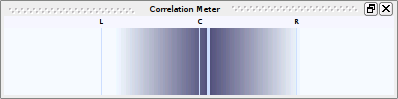
\includegraphics[width=0.7\textwidth]{images/cmeter1}}
	\subfigure[Mono, $r = 1.0$]{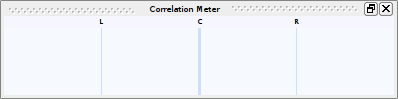
\includegraphics[width=0.7\textwidth]{images/cmeter2}}
	\subfigure[Phase cancellation, $r = -1.0$]{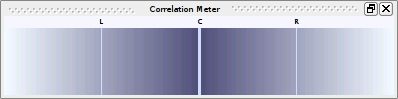
\includegraphics[width=0.7\textwidth]{images/cmeter4}}
	\caption{The correlation meter in Traverso shows the correlation coefficient of the master output signal as a gradient between two lines representing the left and the right channel. If the gradient spreads from L to R, the data is uncorrelated (correlation coefficient $r = 0.0$), and the signal has a wide stereo width (top). If the gradient is collapsed to a line, the data is perfectly correlated ($r = 1.0$), which means the signal is mono (middle). If the gradient spreads beyond the L and R lines, the correlation becomes negative, which means there's a high risk of audible phase cancellations if the output is switched to mono (bottom).}
	\label{fig_cmeter01}
\end{figure}

The correlation meter can also be used to balance the master output. If the levels of the left and right channel are well balanced, the gradient center line should ``wobble'' around the center indicator.

Since the gradient usually occupies the area between the L and R lines, the space outside of the lines is  wasted most of the time. Thus the scale of the correlation meter can be changed by pressing \sact{M}.

\section{FFT spectrum analyzer}
A spectrum analyzer using the fast fourier transformation (FFT) to calculate the spectral power distribution of an audio signal is standard equipment in digital audio workstations. The FFT spectrum analyzer in Traverso can be opened from the menu ``Views $\rightarrow$ FFT Spectrum''. It is a dock window which can either be docked into the main window, or moved freely by dragging with the mouse.

The FFT spectrum analyzer monitors the stereo output channel and decomposes the signal into frequency bands. Each band shows the highest value $dB_{left} + dB_{right}$ in its range (\FigB\ \ref{fig_fft1}). A configuration dialog can be called with \sact{E}, or from the menu opened with \sact{Q} or a right mouse button click.

\begin{figure}
	\centering
	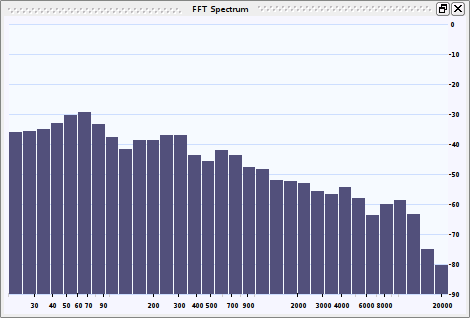
\includegraphics[width=0.6\textwidth]{images/fft1}
	\caption{The FFT spectrum analyzer decomposes the master output signal into its frequencies.}
	\label{fig_fft1}
\end{figure}

The configuration dialog shown in \FigT\ \ref{fig_fft3} allows to define the dB- and frequency range to be displayed. The audible spectrum ranges from 20 to approximately 18000 Hz, whereas CDs range from 20 to 22050 Hz. These are thus recommended values for the lower and upper frequency limit. The upper limit for dB values on the y axis is usually in the range from $-6$ to $+6$ dB, the lower limit between $-60$ and $-120$ dB. The number of bands can be chosen freely, but high numbers ($\geq 128$) cause significantly higher CPU load.

The feature ``show average spectrum'' activates a curve which calculates the average frequency spectrum by accumulating the values as long as Traverso is playing back. The curve is reset if playback is restarted or by the key action \sact{L}. The average curve can also be toggled by the key action \sact{M}, and as soon as there is average data available, the curve can be exported either as raw numbers, or in \texttt{grace} format, which can be opened with the program XmGrace (key action \dact{Return}).

Parameters related to the FFT calculation can be configured in the section ``Advanced Options''. The FFT size determines the lower end of the spectrum; larger FFTs extend to lower frequencies, but cause more CPU load. The lowest frequency captured by the FFT is calculated as:
\[
f_{min} = \frac{\textrm{Samplerate}}{\textrm{FFT size}}
\]
The \emph{lowest} frequency of an FFT of 1024 samples from an audio signal sampled at 44100~Hz is thus 43.1~Hz. Increasing the FFT size to 2048 samples increases the range to 21.5~Hz. The \emph{highest} frequency captured by an FFT is
\[
f_{max} = 0.5 \cdot \textrm{Samplerate}
\]
For audio data sampled at 44100~Hz the upper limit is thus fixed at 22050~Hz.

The windowing function is highly FFT specific and it is beyond the scope of this document to explain it in detail. Users who don't have a particular reason to use a different function are adviced to use the ``Hanning'' window.

\begin{figure}
	\centering
	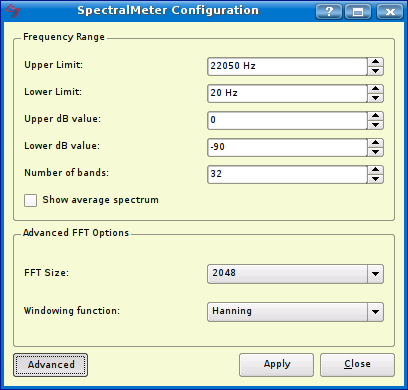
\includegraphics[width=0.7\textwidth]{images/fft3}
	\caption{A configuration dialog called with \sact{E} allows to configure many parameters of the FFT spectrum analyzer.}
	\label{fig_fft3}
\end{figure}

\emph{Note:} For very large FFT sizes the update rate of the spectrum analyzer becomes low. This is not necessarily caused by CPU overload (although CPU load becomes higher for larger FFT sizes), but by the fact that it takes some time to fill the buffers with such large amounts of data. The widget waits until the buffers are full before updating the display.



\chapter{Getting Help\label{sect_help}}
There are several internet resources which can provide help if you struggle with Traverso. Before posting a question, however, it is recommended to carefully classify your problem. The source packages released by the Traverso team are usually well tested and compile without too much tinkering. If you still fail to compile it on your system, the Traverso team will most probably refer you to the user forum of your distribution. You can make life easier for all of us by posting your question there in the first place. Thus we ask you to consider the following points before asking for help.

\section{Compilation fails}
Please make sure that you have installed all required packages listed in chapter \ref{sect_installation} of this document. If you still get the error, search the archive of the Traverso developer mailing list \cite{ml-archive} for the same problem. If you don't find a solution, send an e-mail with a description  and the compiler output attached to the developer mailing list (traverso-devel@nongnu.org) or file a support request on the Savannah project page \cite{support}. Chances are high that the problem is distribution-specific and that you will be asked to refer to the user forum of your distribution.

If you can track down the error to missing dependencies, please consider to seek advice in the distribution forum in the first place.

\section{Binary package fails to install}
Search the archive of the Traverso developer mailing list \cite{ml-archive} for the solution. If you don't find the answer, send an e-mail with an accurate description of the problem to the Traverso developer mailing list (traverso-devel@nongnu.org).

\section{Bugs}
Search the archive of the Traverso developer mailing list \cite{ml-archive} and the bug tracker on Savannah \cite{bugtracker} for discussions of the problem. If you don't find any references, report the bug with instructions for reproduction, relevant information on your hardware, and the version of the Qt library used, on the bug tracker \cite{bugtracker}.

%\section{Feature request}
%Please (!) ask yourself if it is realistic to implement the requested feature at the current stage of development. If yes, send an e-mail with a detailed description to the developer mailing list \cite{ml-archive}.

\section{Getting involved}
The Traverso team highly appreciates any kind of contribution. If you are C++ coder, artist, musician, translator, or bug hunter who wants to help making Traverso the best multitrack application ever, please offer your help on the developer mailing list (traverso-devel@nongnu.org).


\chapter{Troubleshooting}
\begin{itemize}
 \item \textit{Playback is not smooth and I get lots of xruns}\\
  If you are using an Intel onboard sound chip, you may have to set the Number of Periods to 3 instead of 2. This can be done in the ``Audio Driver'' page of the Preferences dialogue, or in your jackd configuration (e.\,g. qjackctl).

 \item \textit{I can't hear anything}\\
  If playback seems to be working (VUMeters indicate a signal), but you hear no sound, check if the ``Null Driver'' is loaded. If yes, load a different driver, e.\,g. ALSA on Linux, or PortAudio on OS X or Windows, and try again. If you are using the jackd driver, make sure the output of Traverso is connected to a hardware output. This is described in chapter \ref{sect_setup}.

 \item \textit{I can't load the driver}\\
  One problem could be that the buffer size specified in the driver settings is too large for your sound card. Try reducing the latency a bit. It can also happen that the sound system is blocked by another application or demon. If you are using KDE, make sure aRTs terminates automatically after a few seconds, and try to shut down any other application blocking the sound card.

 \item \textit{My mouse stops moving when I press a key}\\
  In order to avoid accidental input, some laptops disable the trackpad during key presses. This of course spoils the concept of soft selections completely, but fortunately it can be turned off in most cases. If you are using Linux, the \texttt{mouseemu} demon handles the feature. You can either turn off \texttt{mouseemu} by running the command 
  \begin{verbatim}
  sudo /etc/init.d/mouseemu stop
  \end{verbatim}
  and check if the problem is solved, or you can edit the configuration file \texttt{/etc/defaults/mouseemu} and change the value 300 in the line \texttt{TYPING\_BLOCK="-typing-block 300"} to 0. If there is a comment sign ``\#'' at the beginning of the line, remove it. Then restart \texttt{mouseemu} by typing
  \begin{verbatim}
  sudo /etc/init.d/mouseemu restart
  \end{verbatim}

 If you are using OS X, disable the feature ``ignore accidental trackpad input'' in the system settings.
\end{itemize}



%\appendix
%---------------- End of the document ---------------

\begin{thebibliography}{xx}
   \bibitem{trav-hp}http://www.traverso-daw.org
   \bibitem{trav-repo}deb http://www.traverso-daw.org binary-i386/
   \bibitem{pro-audio-wiki}http://proaudio.tuxfamily.org/wiki/
   \bibitem{suse-ref}http://packman.links2linux.org/package/traverso
   \bibitem{macports}http://www.apple.com/downloads/macosx/unix\_open\_source/macports.html
%   \bibitem{savannah-ref}http://savannah.nongnu.org/projects/traverso/
   \bibitem{ml-archive}http://lists.gnu.org/archive/html/traverso-devel/
   \bibitem{support}http://savannah.nongnu.org/support/?group=traverso
   \bibitem{bugtracker}http://savannah.nongnu.org/bugs/?group=traverso
\end{thebibliography}

\end{document}
